\documentclass{../tuda-beamer}


% Title information
\authors{Simon Hock}
\authors{Nhan Huynh}
\authors{Daniel Mangold}
\date{24. November 2021}

\begin{document}

  \maketitle

  \begin{frame}{Organisatorisches}
    \begin{itemize}
      \item 01.12.2021 Präsenzsprechstunde im Raum in Raum S103/\textbf{103}!
    \end{itemize}
  \end{frame}

  \begin{frame}{Interfaces}
    \begin{itemize}
      \item Schnittstelle: Trennt, was eine Klasse tut, und wie die Klasse es tut
      \item Keine Objekte können instanziiert werden
      \item Zustandslos: Enthält nur Konstanten, Klassenmethoden und nicht implementierte
      Objektmethoden
      \begin{itemize}
        \item Konstante: \inlinejava{static final}
      \end{itemize}
      \item Schlüsselwort: \inlinejava{interface}
      \item Alles im Interface ist implizit \inlinejava{public}
      \item Zusätzlich sind alle Methoden implizit \inlinejava{abstract}
      \item Ausnahme:
      \begin{itemize}
        \item Seit Java 8: Implementierte Objektmethoden mit dem Schlüsselwort \inlinejava{default}
        \item Seit Java 9: Implementierte Methoden mit dem Schlüsselwort \inlinejava{private}
      \end{itemize}
    \end{itemize}
  \end{frame}

  \begin{frame}{Vertrag}
    \begin{minipage}{.475\linewidth}
      \begin{itemize}
        \item Beschreibung der Funktionalitäten
        \item Genauere Implementierung bleibt offen
        \item Entwickler: Freiheit
      \end{itemize}
    \end{minipage}
    \hfill
    \begin{minipage}{.475\linewidth}
      \begin{figure}[ht]
        \centering
        
\begin{tikzpicture}
          \def\width{2.25}
          \def\height{3}
          \draw[fill = white, rounded corners, ultra thick] (0, 0) rectangle (\width, \height);
          \foreach \y in {.5, 1, 1.5, 2, 2.5}{
            \draw[ultra thick] (.35, \y) -- (\width - .35, \y);
          }
          \def\offset{2}
          \begin{scope}[rotate = 330, scale = 0.5, transform shape]
            \fill[yellow!50] (0, 4 + \offset) -- (.4, 4 + \offset)
            -- (.4, 0 + + \offset) -- (.3, - .15 + + \offset)
            -- (.2, 0 + + \offset) -- (.1, -.14 + + \offset)
            -- (0, 0 + + \offset) -- cycle;
            \draw[color = white] (.2, 4 + + \offset) -- (.2, 0 + + \offset);
            \fill[black] (0, 3.5 + + \offset) -- (.2, 3.47 + + \offset)
            -- (.4, 3.5 + + \offset) -- (.4, 4 + + \offset) arc(30:150:0.23cm);
            \fill[brown!40] (0, 0 + + \offset) -- (.2, -.8 + + \offset)
            node[coordinate, pos = .75] (a) {} -- (.4, 0 + + \offset)
            node[coordinate,pos = .25] (b) {} -- (.3, -.15 + + \offset)
            -- (.2, 0 + + \offset) -- (.1, -.14 + + \offset) -- cycle;
            \fill[gray] (a) -- (.2, -.8 + + \offset) -- (b) -- cycle;
          \end{scope}
        \end{tikzpicture}
        \caption{Vertrag}
      \end{figure}
    \end{minipage}
  \end{frame}

  \begin{frame}{Analogie - Schablone}
    \begin{figure}[h]
      \centering
      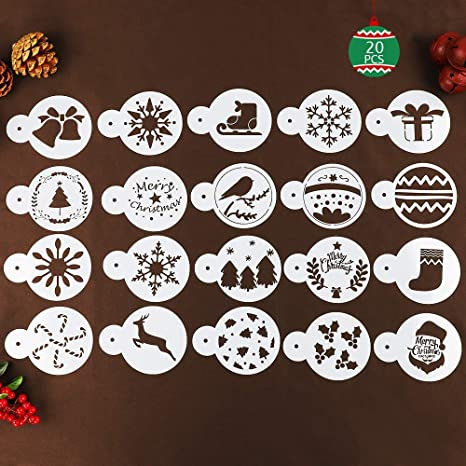
\includegraphics[width=.3\linewidth]{graphics/cookies}
      \caption{\url{https://images-na.ssl-images-amazon.com/images/I/71Fey\%2BGutvL._AC_SX466_.jpg}}
    \end{figure}
  \end{frame}

  \begin{frame}[c]
    \lstinputlisting[style=Java, title=Klasse Ingredient]{codes/Ingredient.java}
  \end{frame}

  \begin{frame}[c]
    \lstinputlisting[style=Java, title=Klasse Recipe]{codes/Recipe.java}
  \end{frame}

  \begin{frame}[c]
    \lstinputlisting[style=Java, title=Interface Cookie]{codes/Cookie.java}
  \end{frame}

  \begin{frame}[c]
    \lstinputlisting[style=Java, title=Klasse ShortbreadBiscuit]{codes/ShortbreadBiscuit.java}
  \end{frame}

  \begin{frame}{Abstrakte Klassen}
    \begin{itemize}
      \item Vorlagen mit Zuständen und Funktionalitäten für Unterklassen
      \item Keine Objekte können instanziiert werden
      \item Kann Attribute enthalten
      \item Kann implementierte und nicht implementierte Objektmethoden enthalten
      \begin{itemize}
        \item Abstrakte Methode mittels Schlüsselwort \inlinejava{abstract}
      \end{itemize}
      \item Beliebige Sichtbarkeiten
      \item Schlüsselwort: \inlinejava{abstract}
    \end{itemize}
  \end{frame}

  \begin{frame}[c]{Beispiel - Sortierung}
    \lstinputlisting[style=Java, title=Interface Sortable]{codes/Sortable.java}
  \end{frame}

  \begin{frame}[c]
    \lstinputlisting[style=Java, title=Abstrakte Klasse ArraySort]{codes/ArraySort.java}
  \end{frame}

  \begin{frame}[c]
    \lstinputlisting[style=Java, title=Klasse ArraySelectionSort]{codes/ArraySelectionSort.java}
  \end{frame}

  \begin{frame}{Nützliche Informationen}
    \begin{itemize}
      \item Ein Interface kann beliebig viele Interfaces erweitern.
      \item Eine Klasse kann nur eine Klasse erweitern (Einfachvererbung) und beliebig viele
      Interfaces implementieren.
      \item Eine Klasse gilt als abstrakt, falls es eine nicht implementierte Methode besitzt.
      \item Nicht implementierte Methoden bei Erweiterungen (Interface und abstrakte Klassen)
      müssen nicht erneut definiert werden.
    \end{itemize}
  \end{frame}

  \begin{frame}[c]{Beispiel - Erweiterung von Interfaces}
    \lstinputlisting[style=Java]{codes/Identifiable.java}
  \end{frame}

  \begin{frame}[c]
    \lstinputlisting[style=Java]{codes/Sortable_Identifiable.java}
  \end{frame}

  \begin{frame}{Klassenattribute}
    \begin{itemize}
      \item Statische Attribute sind Eigenschaften, die nicht einzelnen Objekten, sondern deren
      gesamter Klasse zugeordnet werden.
      \item Schlüsselwort: \inlinejava{static}
      \item Formaler Aufbau: Zugriffsmodifikator\(^+\) \inlinejava{static} Datentyp Bezeichner =
      Wert;
      \begin{itemize}
        \item Die Begriffe, die mit einem \(^+\) (Asterisk) markiert sind, sind optional.
      \end{itemize}
      \item Zugriff: Klassenname.Klassenattribut
    \end{itemize}
  \end{frame}

  \begin{frame}[c]{Beispiel}
    \lstinputlisting[style=Java]{codes/Person_Static.java}
  \end{frame}

  \begin{frame}[c]
    \begin{itemize}
      \item Welchen Namen gibt \inlinejava{joe} zurück?
      \item Welchen Namen gibt \inlinejava{sarah} zurück?
    \end{itemize}

    \lstinputlisting[style=Java]{codes/Person_Example.java}
  \end{frame}

  \begin{frame}{Objektattribute}
    \begin{itemize}
      \item Jede Instanz hat ihre eigenen Objektattribute mit eigenen Werten.
      \item Ohne Schlüsselwort \inlinejava{static}
      \item Formaler Aufbau: Zugriffsmodifikator\(^+\) Datentyp Bezeichner =
      Wert;
      \begin{itemize}
        \item Die Begriffe, die mit einem \(^+\) (Asterisk) markiert sind, sind optional
      \end{itemize}
      \item Zugriff: Objekt.Objektattribut
    \end{itemize}
  \end{frame}

  \begin{frame}[c]{Beispiel}
    \lstinputlisting[style=Java]{codes/Person_Object.java}
  \end{frame}

  \begin{frame}[c]
    \begin{itemize}
      \item Welchen Namen gibt \inlinejava{joe} zurück?
      \item Welchen Namen gibt \inlinejava{sarah} zurück?
    \end{itemize}

    \lstinputlisting[style=Java]{codes/Person_Example.java}
  \end{frame}

  \begin{frame}[c]{Arbeitsphase}
    \begin{center}
      \textbf{\LARGE Selbstständiges Arbeiten}
    \end{center}
  \end{frame}
\end{document}
